\subsection{Introducción}

En el presente ejercicio, se procedió a medir los tiempos de propagación, rise y fall de una compuerta NOR \href{http://www.ti.com/lit/ds/symlink/sn74hc02.pdf}{74HC02}, primero en vacío, luego implementando el siguiente circuito y distintas modificaciones a este:

\begin{figure}[H]
\begin{center}
\begin{circuitikz}

	\node [american nor port](O){};
	\draw (O.in 2) -- (O.in 1);
	\draw ($ (O.in 2) !.5! (O.in 1) $) to[short] ++(-1,0) node[circ, label=left:$V_{in}$](){};
	\draw (O.out) to[short] ++(0.5,0) node[](aux1){};

	\draw (aux1.center) ++(2,3) node[american nand port](A1){};
	\draw (aux1.center) ++(2,1) node[american nand port](A2){};
	\draw (aux1.center) ++(2,-1) node[american nand port](A3){};
	\draw (aux1.center) ++(2,-3) node[american nand port](A4){};

	\draw (A1.in 1) -- (A1.in 2);
	\draw (A2.in 1) -- (A2.in 2);
	\draw (A3.in 1) -- (A3.in 2);
	\draw (A4.in 1) -- (A4.in 2);
	
	\draw (aux1.center) |- ($ (A1.in 2) !.5! (A1.in 1) $);
	\draw (aux1.center) |- ($ (A2.in 2) !.5! (A2.in 1) $);
	\draw (aux1.center) |- ($ (A3.in 2) !.5! (A3.in 1) $);
	\draw (aux1.center) |- ($ (A4.in 2) !.5! (A4.in 1) $);
	
	\draw (A1.out) to[R, l = $1 \ k\Omega$] ++(2,0) to[leDo] ++(1.5,0) node[](aux2){};
	\draw (A2.out) to[R, l = $1 \ k\Omega$] ++(2,0) to[leDo] ++(1.5,0);
	\draw (A3.out) to[R, l = $1 \ k\Omega$] ++(2,0) to[leDo] ++(1.5,0);
	\draw (A4.out) to[R, l = $1 \ k\Omega$] ++(2,0) to[leDo] ++(1.5,0) node[](aux4){};
	\draw (aux2.center) -- (aux4.center){} -- ++(0,-1.5) node[ground](gnd){};

	\draw (aux1.center) |- ++(2,-4.5) to[R, l = $560 \ \Omega$] ++(2,0) to[leDo] (gnd){};
\end{circuitikz}
\caption{Circuito a implementar.}
\label{fig:circuito}
\end{center}
\end{figure}

\subsection{Mediciones a baja frecuencia}

Primero se realizaron las mediciones utilizando un escalón de amplitud $V_{pp}=5 \ V$ con una frecuencia $f=5 \ Hz$, obteniéndose así los siguientes resultados:
\begin{table}[H]
\centering
\begin{tabular}{ccccc}
\hline
Caso & $tpd_{L-H} \ [ns]$ & $tpd_{H-L} \ [ns]$ & trise $[ns]$ & tfall $[ns]$ \\ \hline
Sin carga & 11.10 & 8.75 & 21.0 & 19.0 \\
Con carga & 12.30 & 9.45 & 22 & 19.8 \\ \hline
%Sin carga (100 kHz) & 8.35 & 9.85 & 19.6 & 19.1 \\ \hline
%Con carga (100 kHz) & 12.15 & 9.25 & 20 & 19.4 \\ \hline
%Con carga y capacitores (100 kHz) & 15.85 & 12.60 & 25 & 25.1 \\ \hline
\end{tabular}
\caption{Mediciones obtenidas a bajas frecuencias.}
\label{tb:bf}
\end{table}

Tomando en cuenta las limitaciones presentadas por el osciloscopio disponible en el laboratorio, se puede apreciar que los tiempos medidos se asemejan bastante a los de sus análogos establecidos en la hoja de datos provista por el fabricante. En frecuencias bajas, al conectar la carga ya establecida, se puede apreciar que sus tiempos de operación se incrementan levemente alrededor de $1 \ ns$. 

\subsection{Mediciones a alta frecuencia}
A continuación, se procedió a aumentar la frecuencia de la señal de entrada a $f=100 \ kHz$, repitiendo las mediciones previas, obteniendo los siguientes resultados:
\begin{table}[H]
\centering
\begin{tabular}{ccccc}
\hline
Caso & $tpd_{L-H} \ [ns]$ & $tpd_{H-L} \ [ns]$ & $t_{rise}$ $[ns]$ & $t_{fall}$ $[ns]$ \\ \hline
Sin carga (100 kHz) & 8.35 & 9.85 & 19.6 & 19.1 \\
Con carga (100 kHz) & 12.15 & 9.25 & 20 & 19.4 \\ \hline
\end{tabular}
\caption{Mediciones obtenidas a altas frecuencias.}
\label{tb:af}
\end{table}

En esta última tabla se puede observar que la compuerta tarda más en actuar si se encuentra conectada a una carga. Además, a mayor frecuencia, se puede notar que el integrado tiene un leve aumento en su temperatura, esto se debe a que como debe transicionar con mayor velocidad entre estado alto y bajo, los transistores permanecen mas tiempo en la zona activa, por lo que consumen mayor potencia, manifestándose como el aumento de temperatura previamente mencionado.

\subsection{Mediciones a la tensión de alimentación}
Con el circuito trabajando con una señal de entrada de frecuencia $f=100 \ kHz$, se ve se puede notar que, al realizarse una transición de estados, la alimentación experimenta un sobrepico, seguido de un régimen subamortiguado hasta que vuelve a establecerse después de cierto tiempo. También se puede notar que, antes de dicho sobrepico, la tensión decae por debajo de los $4 \ V$ y aumenta hasta llegar al rededor de los $5.5 \ V$. Este fenómeno ocurre ya que la compuerta le pide más corriente a la alimentación en dichas transiciones. Para solucionar este problema, el fabricante recomienda poner capacitores de desacople de $100 \ nf$ entre las terminales de alimentación del integrado y la del circuito, tratando de que estén lo mas cercanos posibles a dichas terminales. Una vez colocado estos componentes, se puede observar en la Figura (\ref{fig:figuramistica}), una considerable reducción tanto del sobrepico como del tiempo de establecimiento, comparados con los presentados anteriormente.
\begin{figure}[H]
    \centering
    \begin{tabular}{c c}
        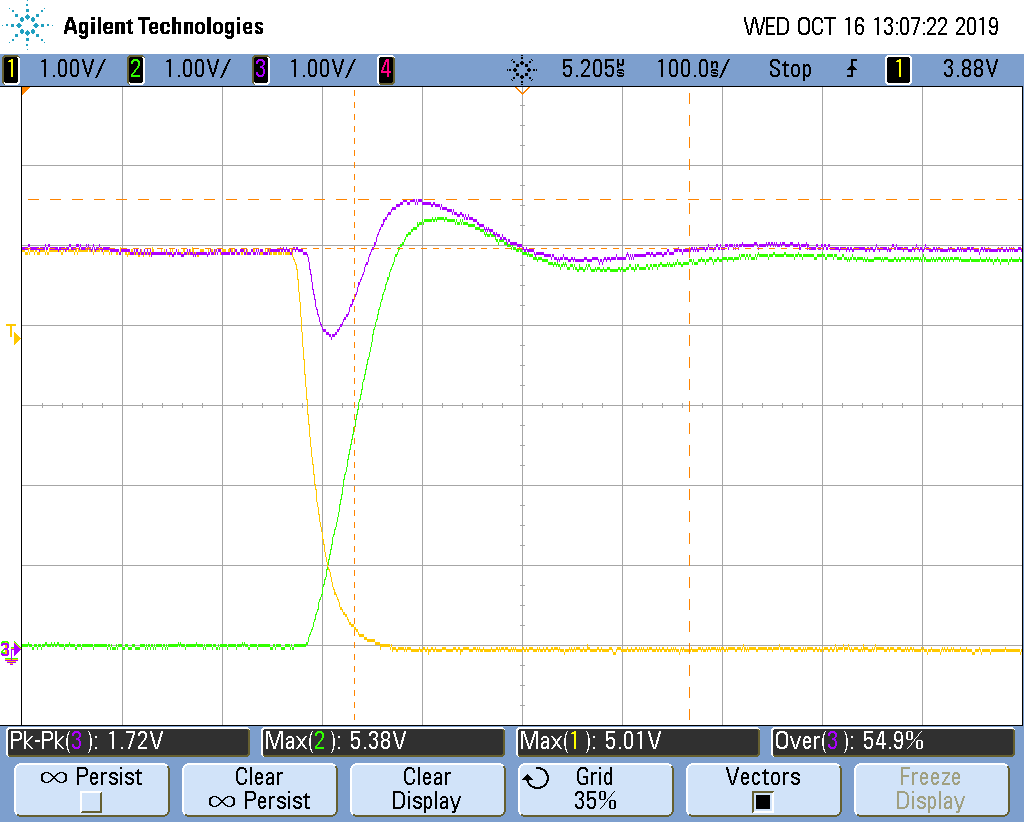
\includegraphics[width=0.4\textwidth,trim={0 2.2cm 0.1cm 1.75cm},clip]{ImagenesEjercicio4/overshoot.png} &
        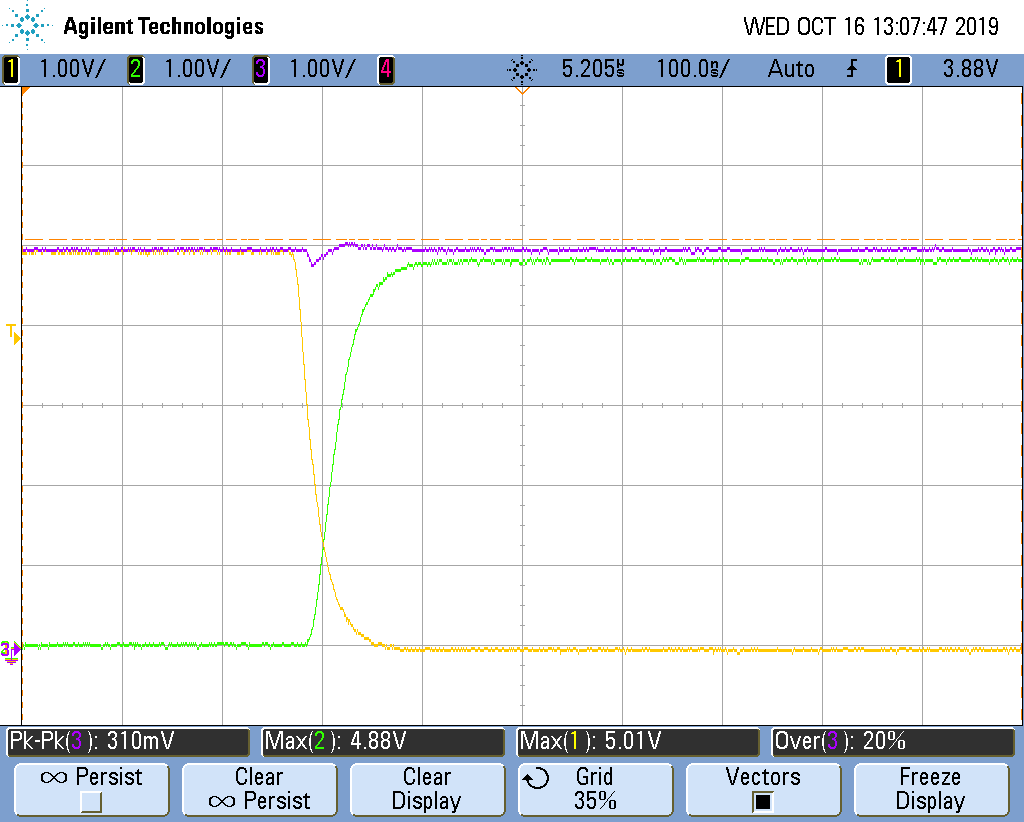
\includegraphics[width=0.4\textwidth,trim={0 2.2cm 0.1cm 1.75cm},clip]{ImagenesEjercicio4/overshoot_c.png}
    \end{tabular}
    \caption{Medición de alimentación primero sin y despues con compensación, en amarillo la señal de entrada, en verde la señal de salida y en azul la alimentación}
    \label{fig:figuramistica}
\end{figure}